\documentclass[12pt]{article}
\usepackage{graphicx}
\usepackage[none]{hyphenat}
\usepackage{graphicx}
\usepackage{listings}
\usepackage[english]{babel}
\usepackage{graphicx}
\usepackage{caption} 
\usepackage{booktabs}
\usepackage{array}
\usepackage{amssymb} % for \because
\usepackage{amsmath}   % for having text in math mode
\usepackage{extarrows} % for Row operations arrows
\usepackage{listings}
\lstset{
  frame=single,
  breaklines=true
}
\usepackage{hyperref}
  
%Following 2 lines were added to remove the blank page at the beginning
\usepackage{atbegshi}% http://ctan.org/pkg/atbegshi
\AtBeginDocument{\AtBeginShipoutNext{\AtBeginShipoutDiscard}}
\usepackage{gensymb}


%New macro definitions
\newcommand{\mydet}[1]{\ensuremath{\begin{vmatrix}#1\end{vmatrix}}}
\providecommand{\brak}[1]{\ensuremath{\left(#1\right)}}
\providecommand{\sbrak}[1]{\ensuremath{{}\left[#1\right]}}
\providecommand{\norm}[1]{\left\lVert#1\right\rVert}
\providecommand{\abs}[1]{\left\vert#1\right\vert}
\newcommand{\solution}{\noindent \textbf{Solution: }}
\newcommand{\myvec}[1]{\ensuremath{\begin{pmatrix}#1\end{pmatrix}}}
\let\vec\mathbf


\begin{document}

\begin{center}
	\title{\textbf{Quadratric Programming}}
\date{\vspace{-5ex}} %Not to print date automatically
\maketitle
\end{center}
\setcounter{page}{1}

\section{12$^{th}$ Maths - Chapter 6}
This is Problem-23 from Exercise 6.6 
\begin{enumerate}
	\item Find the equation of the normal to the curve $x^2=4y$ and passing through the point $(1,2)$.

\solution 
The given equation of the curve can be written as  
\begin{align}
	\label{eq:parabolaEq2}
	g\brak{\vec{x}} = \vec{x}^T\vec{V}\vec{x} + 2\vec{u}^T\vec{x} + f = 0 
\end{align}
where
\begin{align}
	\label{eq:eqV}
	\vec{V} &= \myvec{ 1 & 0 \\ 0 & 0} \\
	\label{eq:eqU}
	\vec{u} &= \myvec{0 \\ -2} \\
	\label{eq:eqF}
	f &= 0 
\end{align}
We are given that 
\begin{align}
	\vec{h} &= \myvec{1 \\ 2}
\end{align}
This can be formulated as optimization problem as below:
\begin{align}
	\label{eq:Eq3}
	&  \min_{\vec{x}} \quad \text{f}\brak{\vec{x}} = \norm{\vec{x}-\vec{h}}^2\\
	\label{eq:Eq4}
	& \text{s.t.}\quad g\brak{\vec{x}} = \vec{x}^T\vec{V}\vec{x} + 2\vec{u}^T\vec{x} + f = 0  
\end{align}
First we show that, \eqref{eq:Eq4} is not convex. Suppose 
    $\vec{x_1}$ and $\vec{x_2}$ satisfy $g\brak{\vec{x}} = 0$. Then, 
\begin{align}
        \vec{x_1}^\top\vec{Vx_1} + 2\vec{u}^\top\vec{x_1} + f &= 0 \label{eq:x1-parab} \\
        \vec{x_2}^\top\vec{Vx_2} + 2\vec{u}^\top\vec{x_2} + f &= 0 \label{eq:x2-parab}
\end{align}
Then, for any $0 \le \lambda \le 1$, substituting
\begin{align}
       \vec{x_\lambda} \leftarrow \lambda\vec{x_1} + \brak{1-\lambda}\vec{x_2}
\end{align}
into \eqref{eq:Eq4}, we get
\begin{align}
        g\brak{\vec{x_\lambda}} = \lambda\brak{\lambda-1}\brak{\vec{x_1}-\vec{x_2}}^\top\vec{V}\brak{\vec{x_1}-\vec{x_2}} + f \neq 0
        \label{eq:nonconvex}
\end{align}
Hence, the optimization problem is nonconvex. The constraints throw an error when \textit{cvxpy} is used. 

We will use Lagrange multipliers method to find the optimum value. Define
\begin{align}
	H\brak{\vec{x}, \lambda} &= f\brak{\vec{x}} - \lambda g\brak{\vec{x}} 
\end{align}
and we find that 
\begin{align}
	\nabla f\brak{\vec{x}} &= 2\brak{\vec{x}-\vec{h}} \\
	\nabla g\brak{\vec{x}} &= 2\brak{\vec{V}\vec{x}+\vec{u}}
\end{align}
We have to find $\lambda \in \mathbb{R}$ such that
\begin{align}
	&\nabla H\brak{\vec{x},\lambda} = 0 \\
        \label{eq:Eqlambda}
	&\implies 2\brak{\vec{x}-\vec{h}} - 2\lambda\brak{\vec{V}\vec{x}+\vec{u}} = 0 \\
        \label{eq:Eqx}
	&\implies \vec{x} - \vec{h} =  \lambda\brak{\vec{V}\vec{x}+\vec{u}}   \\
	&\implies \brak{\vec{I} - \lambda\vec{V}}\vec{x} =  \lambda\vec{u}+\vec{h} \\ 
	&\implies \myvec{1-\lambda & 0 \\ 0 & 1}\vec{x} = \lambda\myvec{0 \\ -2} + \myvec{1 \\2} \\ 
        \label{eq:EqL}
	&\implies \myvec{1-\lambda & 0 \\ 0 & 1}\vec{x} = \myvec{1 \\ -2\lambda+2}  
\end{align}
We have 2 cases to considers here.
\begin{enumerate}
\item When $\lambda \ne 1$. Writing augmented matrix,
\begin{align}
	&\myvec{1-\lambda & 0 & 1\\ 0 & 1 & -2\lambda+2} \xleftrightarrow[]{R_1 \leftarrow \frac{R_1}{1-\lambda}} \myvec{1&0&\frac{1}{1-\lambda}\\0&1&-2\lambda+2}
\end{align}
Then, we get
\begin{align}
        \label{eq:Eqxm}
	\vec{x}_{m} &= \myvec{ \frac{1}{1-\lambda} \\ -2\lambda+2}
\end{align}
Substituring this value in \eqref{eq:Eq4}
\begin{align}
	&\myvec{\frac{1}{1-\lambda} & -2\lambda+2}\myvec{1 & 0 \\ 0 & 0}\myvec{\frac{1}{1-\lambda} \\ -2\lambda+2} + 2\myvec{0 & -2}\myvec{\frac{1}{1-\lambda}} = 0 \\ 
	&\implies \myvec{\frac{1}{1-\lambda} & 0}\myvec{\frac{1}{1-\lambda} \\ -2\lambda+2} - 4\brak{-2\lambda+2} = 0 \\
	&\implies 8\brak{\lambda^3 -3\lambda^2+3\lambda-1} +1 = 0 \\ 
	&\implies \brak{\lambda^3 -3\lambda^2+3\lambda-1}  = -\frac{1}{8} \\ 
	& \implies \brak{\lambda-1}^3 = -\frac{1}{8} \\ 
	& \implies \lambda-1 = -\frac{1}{2} \\
	& \implies \lambda = \frac{1}{2}
\end{align}
Substituting the value of $\lambda$ in    \eqref{eq:Eqxm}
\begin{align}
	\vec{x}_{m} &= \vec{q} = \myvec{ \frac{1}{1-\frac{1}{2}} \\ -2\frac{1}{2}+2} \\
	&= \myvec{2 \\ 1}
\end{align}
\item When $\lambda = 1$. 
\begin{align}
	\eqref{eq:EqL} \implies \myvec{0 & 0 \\ 0&1}\vec{x} = \myvec{1 \\ 0}
\end{align}
This is an invalid solution. 
\end{enumerate}
Given the point of contact $\vec{q}$, the equation to the normal is given by
\begin{align}
	&\brak{\vec{V}\vec{q}+\vec{u}}^\top\vec{R}\brak{\vec{x}-\vec{q}} = 0 \\
	&\implies \brak{\myvec{1&0\\0&0}\myvec{2\\1}+\myvec{0 \\ -2}}^\top \myvec{0&1 \\-1&0}\brak{\vec{x}-\myvec{2\\1}} =0\\
	&\implies \myvec{2&-2} \myvec{0&1 \\-1&0}\brak{\vec{x}-\myvec{2\\1}} = 0 \\
	&\implies \myvec{2&-2} \myvec{0&1 \\-1&0}\brak{\vec{x}-\myvec{2\\1}} = 0 \\
	&\implies \myvec{1&1}\vec{x} = 3 
\end{align}
The relevant figure is shown in \ref{fig:Fig1}
\begin{figure}[!h]
	\begin{center}
		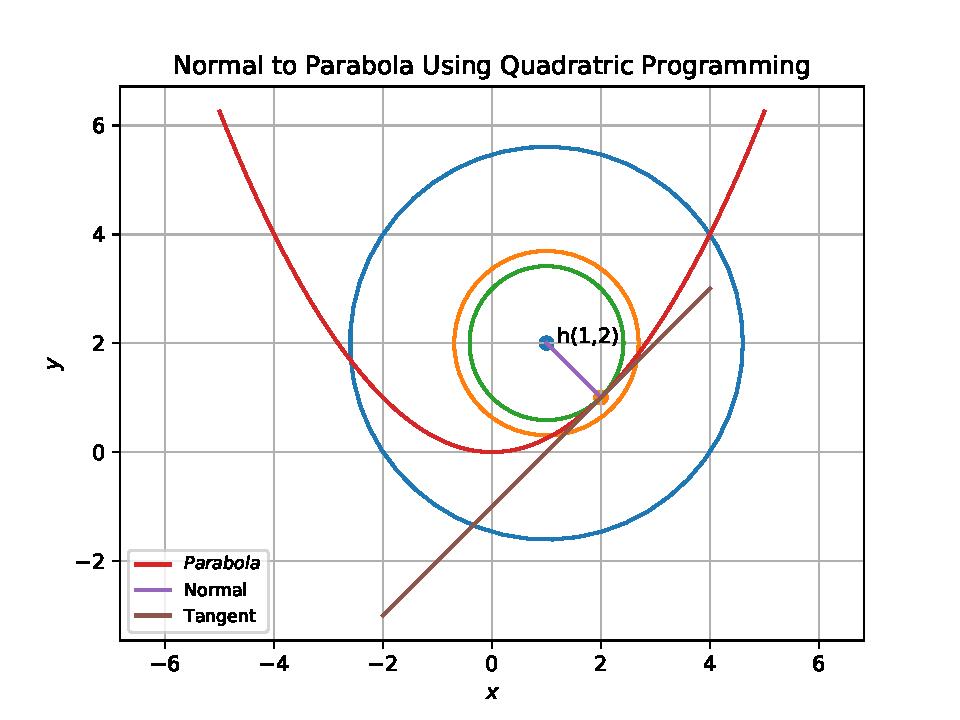
\includegraphics[width=\columnwidth]{figs/problem23.pdf}
	\end{center}
\caption{}
\label{fig:Fig1}
\end{figure}
\end{enumerate}
\end{document}
